\section{SIMULATION RESULTS}

The proposed strategy is implemented and tested using the Robot Operating System (ROS) framework. Our decentralized strategy is compared with the coordinated strategy described in \cite{Burgard2005}. %Describe Burgard here

\begin{figure}[b]
    \centering
	\begin{minipage}{1.0\columnwidth}
	   \centering
	   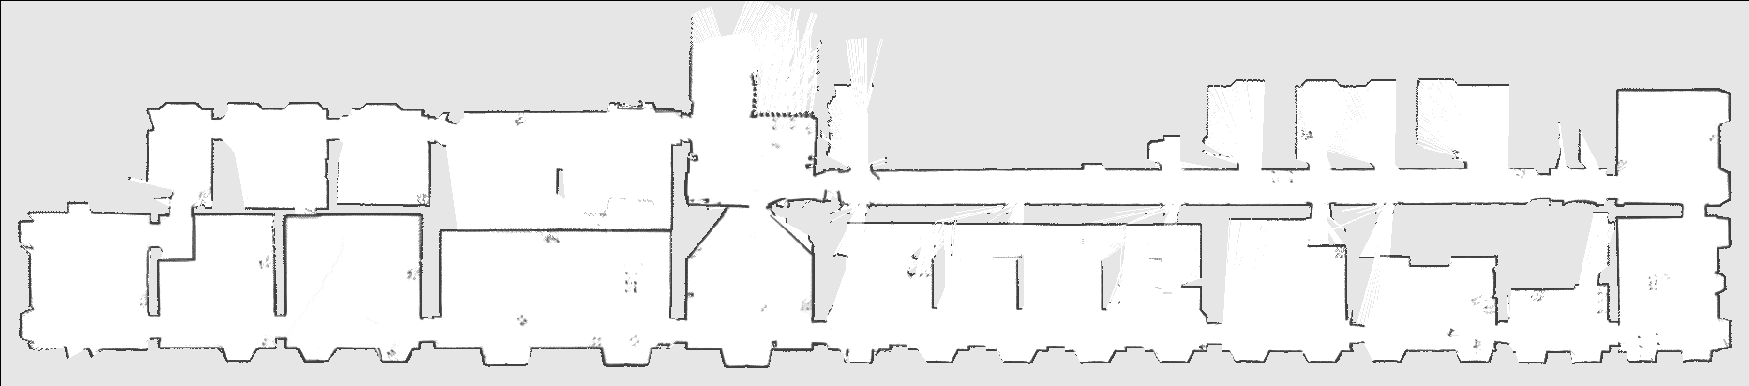
\includegraphics[width=\columnwidth]{./Pictures/belgioioso.pdf}
	   \caption*{a)} 
	\end{minipage}
\hfill 	
	\begin{minipage}{1.0\columnwidth}
	   \centering
	   
\includegraphics[width=\columnwidth]{./Pictures/map.pdf}
	   \caption*{b)} 
	\end{minipage}
\caption{Maps used for simulation experiments. a) Original map: Map from \cite{fr_dataset}. b) Google Cartographer map: The map generated using Google Cartographer SLAM algorithm with previous hand corrections at incomplete parts of the original map.}
\label{scenario}
\end{figure}
We implemented coordinated Burgard's algorithm so that the cost of reaching the frontier point is also proportional to the Euclidean distance between the robot and that point and the utility of a frontier point depends on the number of robots that are moving to that point. Each point is eventually a cell of an occupancy grid map (represents the environment) that contains a numerical value and describes if the corresponding area in the environment is covered by an obstacle or not. The cell are then classified as occupied or free. The frontier detector and filter module are the same for both algorithm implementations (coordinated Burgard's and our decentralized). 


\subsection{Simulation Setup}
Simulations were carried out using the Stage simulator \cite{stageweb}, which provides realistic robot movements inside the loaded environment image. The ROS Navigation stack is used to control and direct the mobile robots towards exploration goals. 
Scenario used in the simulation is Belgioioso Castle, available in \cite{fr_dataset} and shown in Figure \ref{scenario}. It is a challenging and a typical office like scenario with a free space area of approximately 225 ${m}^2$. For the simulation, we use a model of Pioneer P3-DX with maximum speed of 1.3 m/s, laser range 20 m and 360$^{\circ}$ laser scan window. 
We tested the algorithms with teams of two, three and five mobile robots. The number of mobile robots is in our case limited because of the complex simulation setup and computational requirements. Thus we use the appropriate size of the simulation scenario. The robots start off in random positions within this world. The results are presented as average of 10 runs for each set. Constants $\lambda_{u}$, $\lambda_{f}$, $r$ and $r_{f}$ are experimentally determined and set to  0.9, 1.2, 0.5, 3.0 respectively.

\begin{figure}[t]
    \centering
	\begin{minipage}{1.0\columnwidth}
	   \centering
	   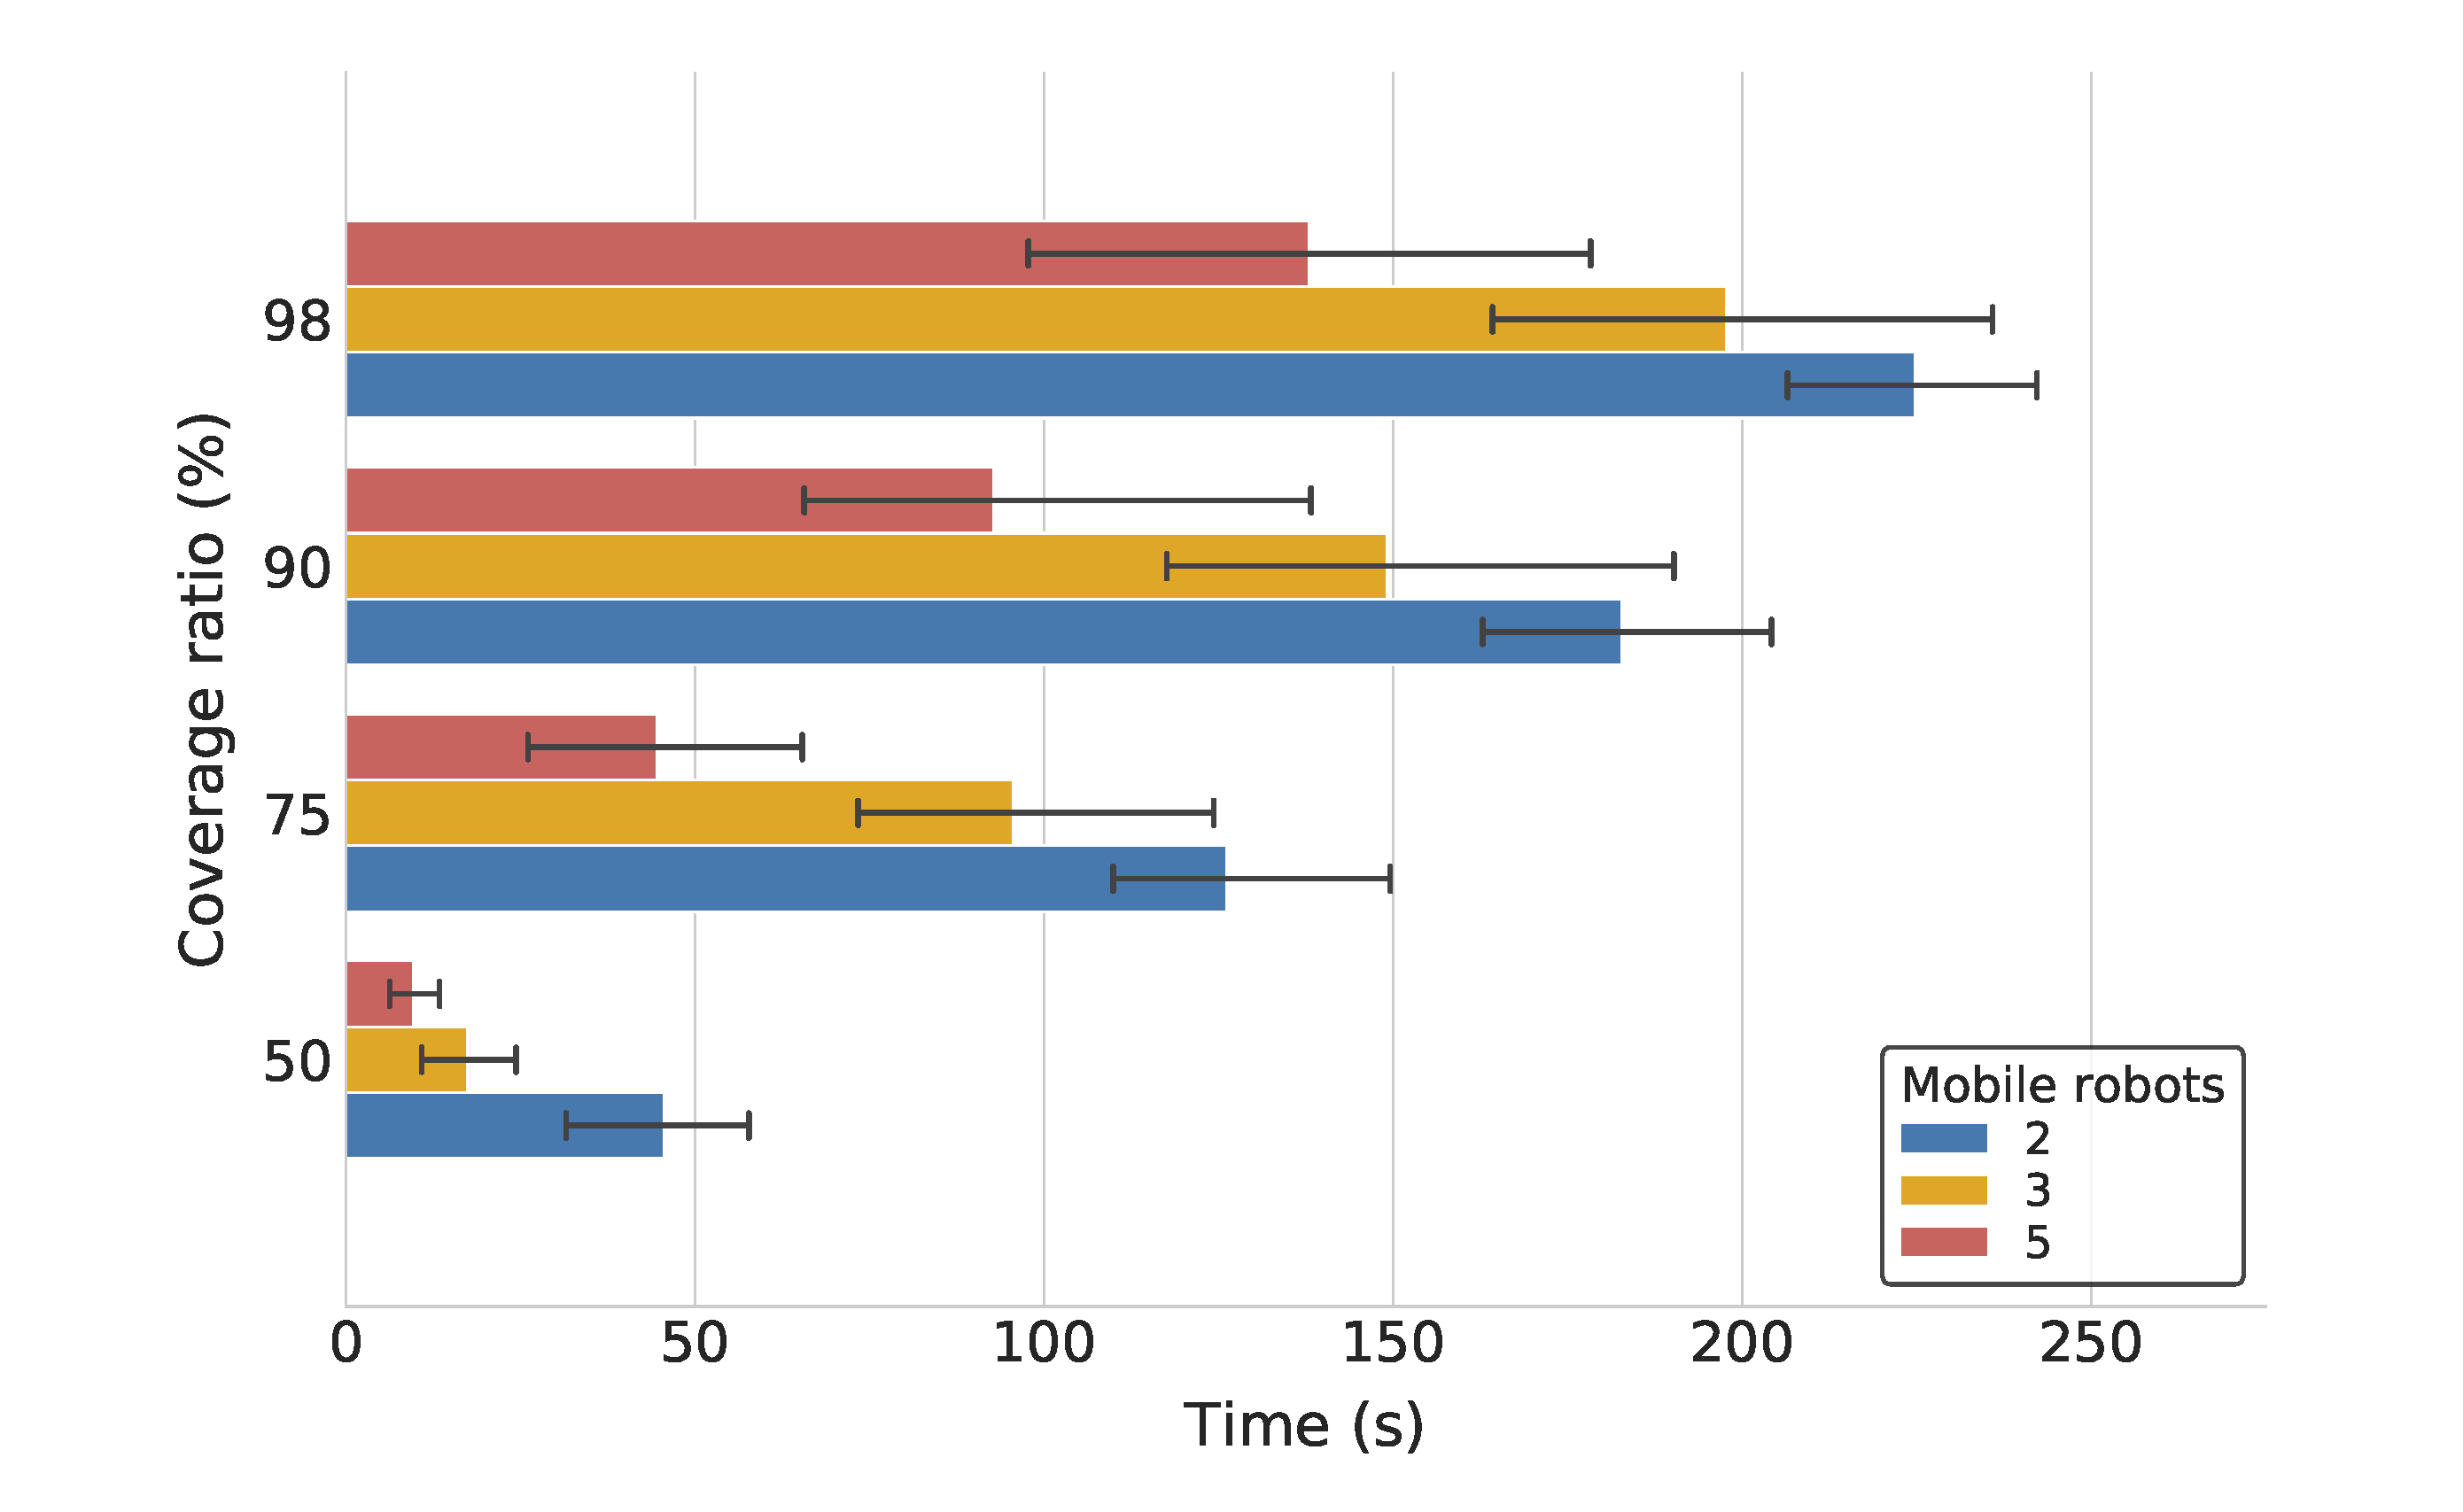
\includegraphics[width=\columnwidth]{./Pictures/burgard_results.pdf}
	   \caption*{a)} 
	\end{minipage}
\hfill 	
	\begin{minipage}{1.0\columnwidth}
	   \centering
	   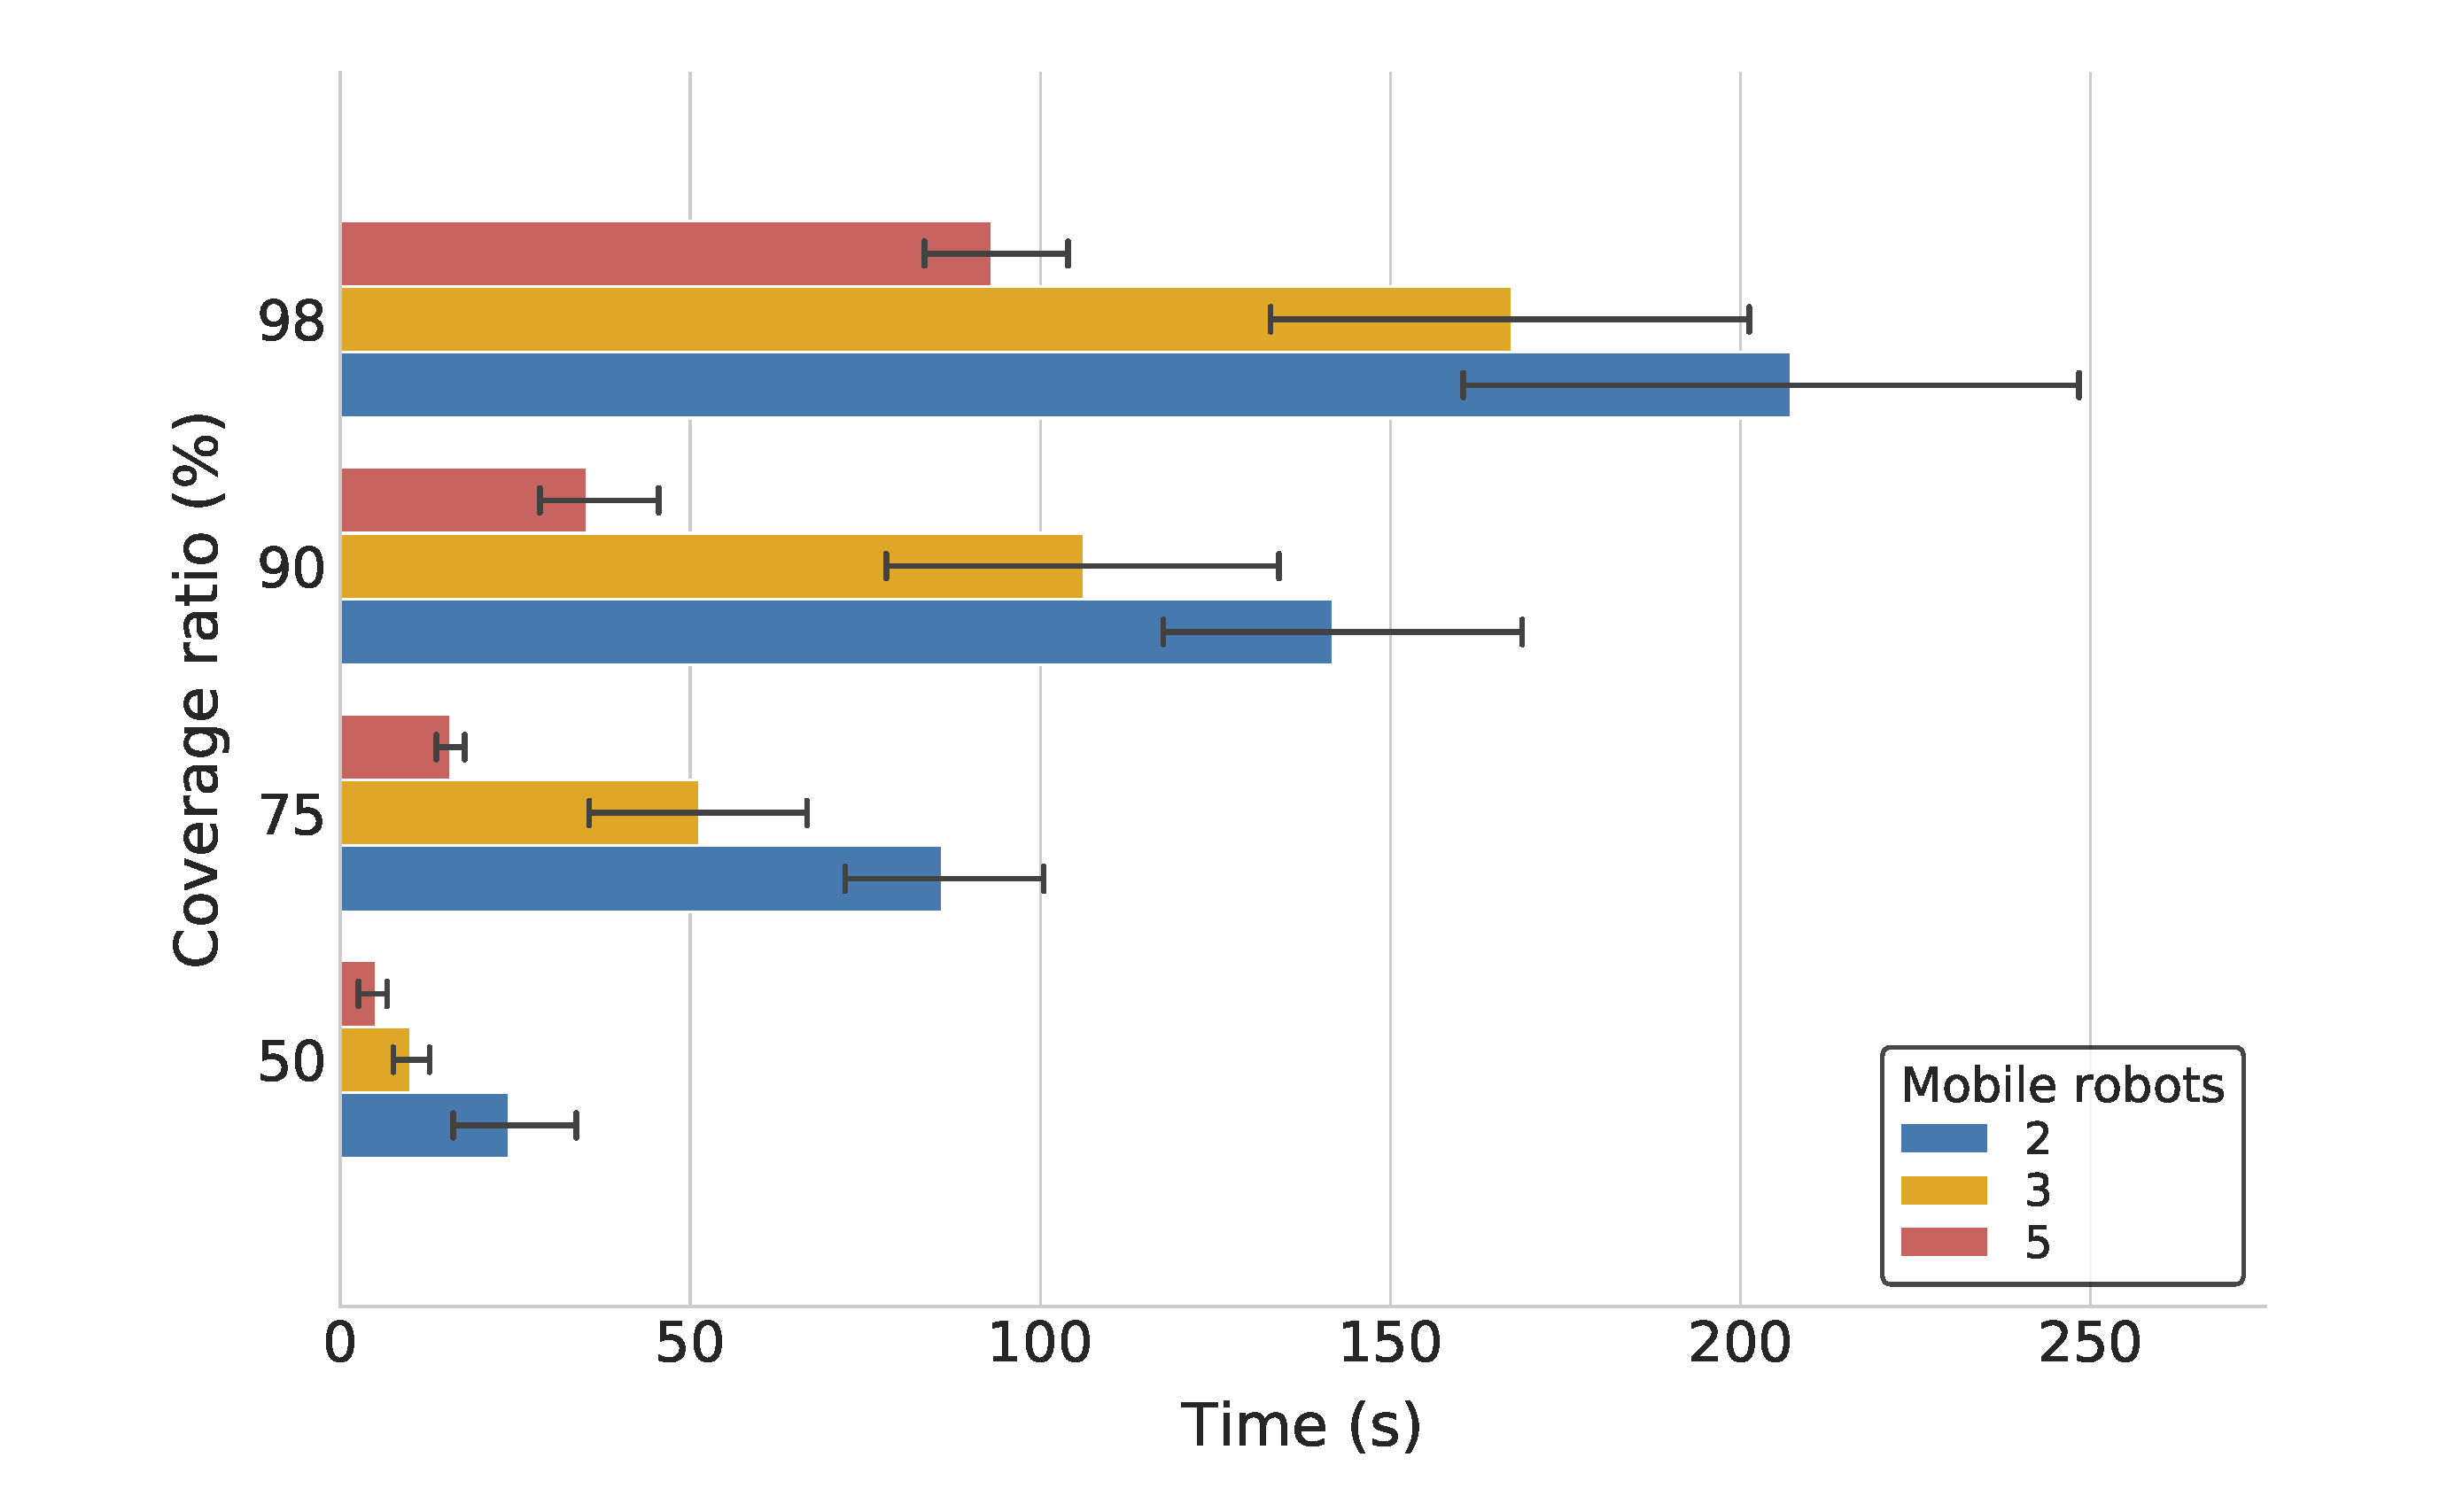
\includegraphics[width=\columnwidth]{./Pictures/decent_results.pdf}
	   \caption*{b)} 
	\end{minipage}
\caption{Simulation results for a) coordinated Burgard's and b) decentralized strategy tested on two, three and five mobile robots.}
\label{fig:results}
\end{figure}


\subsection{Simulation Results}

During the exploration and mapping process covered area in time is recorded. The comparison of the coordinated Burgard's strategy and our decentralized strategy is shown in Fig. \ref{fig:results} using an indicator called \textit{Coverage Ratio (CR)} which addresses percentage of the accessible terrain covered by the mobile robot team. It is calculated as:  \( \frac{\text{explored cells} \cdot 100}{\text{accessible cells}} \).

First of all, it is interesting to see how the coverage evolves over time. Fig. \ref{fig:results} shows \textbf{CR} over time for both coordinated Burgard's and decentralized multi-robot exploration strategies in the described scenario. We report the time it takes to cover 50, 75, 90 and 98 percent of the environment. In the both scenarios, our decentralized strategy needed less time to explore the same percentage of the environment. Furthermore, increase in performance was greater for larger number of mobile robots. Using our decentralized strategy, it took \textbf{7.8 \% , 15.3 \% and 32.6 \%} less time for two, three and five mobile robots respectively to explore the environment compared to coordinated Burgard's strategy. This results show that our decentralized strategy performs significantly better than coordinated Burgrad's, especially for five mobile robots.

When we compare the average exploration time for the both strategies it shows that three mobile robots performs better than two, as well as having five mobile robots instead of three. An area size plays an important role in the optimal number of mobile robots. Due to the relative small scenario and laser range, we assume that more mobile robots will make the area overcrowded. Video recordings for simulation with five mobile robots can be found on \cite{playlist}.

